\documentclass[tikz]{standalone}
\usepackage{pgfplots}
\pgfplotsset{compat=1.15}
\usepackage{mathrsfs}
\usetikzlibrary{arrows,calc}
\usepackage{tkz-euclide}

\pagestyle{empty}

\definecolor{AngleClr}{rgb}{0,0.39215686274509803,0}
\definecolor{ShapeClr}{rgb}{0.6,0.2,0}
\definecolor{BlueClr}{RGB}{5,81,163}

\begin{document}

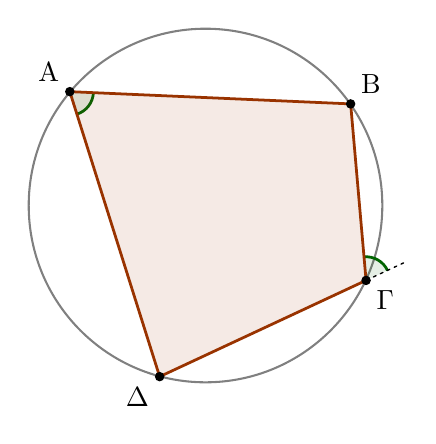
\begin{tikzpicture}[scale=.75]
\tkzSetUpLine[line width=1pt,color=black]
\tkzSetUpPoint[fill=black]

\tkzDefPoint(140:3){A}
\tkzDefPoint(35:3){B}
\tkzDefPoint(-25:3){C}
\tkzDefPoint(-105:3){D}
\tkzDefPointOnLine[pos=1.2](D,C)\tkzGetPoint{E}

\tkzDefTriangleCenter[circum](A,B,C) \tkzGetPoint{O}

\tkzDrawCircle[line width=0.75](O,A)

\tkzFillAngles[fill=AngleClr,size=.4,fill opacity=0.1](D,A,B E,C,B)
\tkzMarkAngles[line width=1pt,color=AngleClr,size=.4](D,A,B E,C,B)

\tkzDrawSegments[line width=0.5pt,color=black,dashed,dash pattern=on 1pt off 1.75pt](D,E)

\tkzFillPolygon[fill=ShapeClr,fill opacity=0.1](A,B,C,D)
\tkzDrawPolygon[color=ShapeClr](A,B,C,D)

\tkzDrawPoints[size=3](A,B,C,D)
\tkzLabelPoint[above left](A){$\rm A$}
\tkzLabelPoint[above right](B){$\rm B$}
\tkzLabelPoint[below right](C){$\rm \Gamma$}
\tkzLabelPoint[below left](D){$\rm \Delta$}

\end{tikzpicture}

\end{document}
